\chapter{Background \& Objectives}

\section{Background}
\subsection{Background and Preparation}
Background research was compromised of analysing existing systems like the original Access Aber, previous work completed by the developer that used map technology within Android and general research into the map technology to gather a strong understanding of exactly what was possible.

A majority of time was spent analysing Access Aber and the currently existing criticisms of it, a lot of the problems were clear without the user feedback that had been provided but some criticisms were more subtle but easy to understand like how the application provides no main menu as such causing the user to feel lost from the start. It was also obvious that at a technical level, the included features were not overly complex, at least not to complete on the Android platform. Due to the application originally being developed on a system which allowed it to be run both on iOS and Android there probably were limitations from both sides which leads to having to develop around the weak elements in both platforms. As stated developing for a single platform should help us avoid these problems while also giving us the ability to take advantage of what is there. Due to this a large amount of research was completed into both UI design within Android as well as the technical benefits both Open Street Maps and Google Maps could provide the development. 

Research was also completed into exactly how the mesh of locations would be created and represented, within the design specification it was concluded that a searchable graph was a possible solution and one worth researching further. This also meant analysing how other existing applications had mapped roads to graphs and the general area of map representation. While this gave a fair amount of answers further decisions needed to be made on both how to search the constructed graph and how to make it an extendible system for future additions. This was one of the main conditions brought up in meetings with the original 'customers' of the Access Aber application, it had to be functional after the initial developers had left. It was also described that it would be beneficial for the application to be developed in such a way that a possible future development that involved a central file store of the information for ranging versions of the application. Due to this further research was done on how we could leave the application in such a way that it facilitated the addition of this feature possibly without using it upon the current cycles completion. 

Past work by the developer was also analysed for anything of use that may come out of it, the application analysed was proven to have functional working code and as such was a place where possible solutions could be found. This included implementation of maps in an Android environment, the logging of a route which is something that has been previously outlined as a key requirement and a fair amount of small features relating the monitoring of a users location and the information which can be gathered from that. Most information gathered from this however was fairly irrelevant, it was decided it was not the best place for referencing in future. 

Finally the Android API and several Android libraries were examined for the benefits they could provide the development with, along with the search for several features that had already been selected for inclusion within the application. This ranged from simple research on Expandable List Views to research on the best way to present the application in an intuitive way, a lot of factors were gathered from the original feedback which guided a lot of the research. While a slide function for the screens was visually appealing the possibility of it confusing users was something that removed it as a possibility very quickly. Research was also performed into Google's Material Design program, a set of guidelines for good design within the Android environment. It contained a large amount of information relating to designing professional and good looking applications, while the information was too much to be fully applied in the projects time line some key ideas were taken from it relating to the design of elements within an application and general theme layout. Furthermore some sites were analysed for basic colour themes and how to implement a simplistic design without it looking unprofessional.
\subsection{Interests}
This project has been chosen due to a variety of reasons, revolving around both the developers interests and the possibility of the project leading to something that can have real world influences. The main source of interest is that the project allows for a development environment that takes input from the real world, mobile devices are of a great deal of interest to the developer due to the data that can be gathered from them and the manipulation of this data. Mobile devices are steadily changing the way we live, with applications that not only help us find where to go but tell us what we can do when we get there. Where other people have liked and even what is best suited to us based on past choices we have made and the device has noted. While some systems outside of mobile development clearly have massive real world influences it is felt by the developer that the easy entry and possibilities provided with mobile development make it one of the most accessible and revolutionary platforms.

With the application in concern providing information to the user it also means we can filter what information is shown based on user details. If the user says i cannot manoeuvre stairs for whatever reason, we could implement a function to provide paths with no stairs, this could obviously be expanded to include searching based on a range of filters. This could also be condensed down to a single graph, with different links becoming available with different information. This kind of possibility is what makes mobile such an interesting platform, not only can we show a map and a route through it, we can then guide a user through it, even ask them for information regarding it once they are done. Possibilities provided are wide and interesting, with so many choices available the future of the application is impossible to predict because of the many paths it could possibly follow.

Another source of interest is the real effect this application could have for an organisation such as Aberystwyth University, the confusing and difficult to traverse campus is not a problem that can be resolved easily. With everything on campus set in stone it is simply not possible to move buildings and locations around. However with technology we can facilitate the use of campus without any physical additions to it at all. This means we can change the physical use of something with technology that does not itself directly effect or control the environment it is deployed in. An interesting possibility would be to examine users manoeuvring of campus before the application is introduced and afterwards, as well as the effect it has on how comfortable disabled users feel on campus. With the application very literally changing the way a user traverses the campus it is possible that some of the more unused walkways could become more travelled due to their inclusion in the application. Further research will have to be done on most effective travel paths around campus, it is likely that the ones currently most travelled are the quickest but that is not definite. 
\section{Analysis}
A broad analysis of the problem with the currently existing Access Aber application is that while it provides solutions, they are long, problematic and make the user follow a convoluted process that may not be obvious to the common person, the exact person we are aiming to help with the application. A prime example of the problems posed is in the route finding within the application, it exists but requires the user to scroll through a huge list of possible routes and then takes them to a summary screen before finally letting the user see the route they need to walk. There are some very obvious, stand out ways, that this can be improved including the implementation of simple features like drop-down boxes for destinations and the removal of the summary screen. 

Most of the problems in the application come from simple solutions to more complex problems, simple in the way that they do not fully cover the problem or provide a real benefit to the system. This appears throughout the application and based on the information provided seems to have been caused by the short time period it was developed in. One aim for this project is to provide a much more polished result with each problem solved properly rather than meeting requirements with a 'it will suffice' mentality. 

Access Aber's initial form will be treated as a kind of groundwork for development, while no code will actually be taken from it the features will be adapted and built upon. This way we can build not only a port of the application to Android we can build a better version which in turn can act as ground work for any future work on the project, be it with the Android application or another new version on another platform. Having this groundwork and the feedback on it means that the some of the problems that need fixing are already highlighted for us, while the time line of the project may not be long enough for some of the features to be fixed most can at least be addressed. 

A step by step guide which details various information such as major features and activities can be seen in the Design Specification (Section 2). The following requirements are what has been decided as key to the success of the application, they have been selected due to either their use to the user or the fact that they have always been included in the project and these aim to be improved versions. 
\subsection{Breakdown of Requirements}
After much analysis the problem has been broken down into a set of requirements, some of the process to arriving at this point can be found in both the Requirements specification with further information in the Design Specification, however the reasoning will be fully discussed here. Each requirement will serve as a benchmark for the project, requirements were set as realistically as possible considering the time given and the work that needs to be completed. 
\subsubsection{Route Finding}
Route finding is seen as by far the major feature within the application, not only is it the most technologically advanced it is also the most useful for our prospective users. As detailed, a graph system had been highlighted as the best way to achieve a representation of campus for us to apply a search algorithm to, with Breadth First Search (BFS from now) seen as a possible solution for the time being. This feature also has some planned extensions to it, firstly the path shown to the user should contain extra information pertaining to the path. This includes information about the difficulty of the route and features along the route such as stairs, it would be beneficial to have information for separate segments beyond their rating but this is a stretch goal and not something should realistically be expected. Due to the expected structure of the graph the implementation of displaying rating of segments within the paths should be attainable, with large routes being made up of many links between nodes it is almost to be expected in a system such as this. 

It is key that the route finding solution be easily expandable, this is due to the maintainability of the application being key to its success. There is no guarantee that the original developer will be around for future expanding if the application is deemed fit for purpose and further developed, due to this it must be possible for the adding of new locations to be possible. An ideal solution would use a central file store to pull location information from, however the problem here which has been previously covered is that there is no guarantee the user has access to internet when using the application. Due to this a sufficient solution should see that the extending of route finding should be achievable by a novice programmer, ideally a common user if they are provided with clear instructions. A set of guidelines should be produced if the project is taken further. 

A further stretch goal would be an implementation of route finding based on a sort of filter, whether this be a routes rating or features on the route. A current rough idea of this can be found in the Design Specification (2.1.1), this highlights the idea of using a separate graph altogether, this way if we make the search algorithm so that all it needs is a set of files in a set way we can have a variety of graphs present within the application. An ideal solution would use a consolidated graph, with different routes between different Nodes being considered, however this is seen as problematic in the current time frame. 

A final possible addition, though not likely to be achievable in the time frame, is to provide access from anywhere to somewhere on campus. This means having a user be guided into the graph from areas outside of it, meaning dynamic routes would have to be created. Initial research shows this could be possible using the Google Directions API however it is likely that with other development ongoing this is likely to be feature developed outside of the initial time frame. However the use of this feature would be a real benefit for the application, a simplistic solution would have the user guided to the nearest node and then the search algorithm would take it from there. It is even possible that in future the whole graph would be replaced with the Directions API, this however would require the user to have access to the internet at all times and it is simply something that cannot be guaranteed. Due to this the hard coded graph and search related to the graph is likely to be present for the lifetime of the application due to the required off line capabilities. 
\subsubsection{Route Plotting}
This desired features comes as a result of the original meetings, the 'customers' were unhappy with the current system of plotting routes, which were all done manually.  Part of the solution is already achieved through the use of a graph, a location only needs to be linked to one other to have a route available to anywhere on the graph. However this should be further developed for the application to be seen as fully functional. The application should include a feature that lets a user log a route and have it printed out to a file compatible with the current route finding solution, this way the person responsible for the future maintenance of the application can visualize a route before they add it to the current system. A route should be able to be visualized while it is being created, so that the user is not blindly adding points. GPS co ordinates received from some devices can be far from where the actual user is. Functionality within the Google Maps API allows us to show the user where the phone thinks they are, this should help them plot accurate points. 

The output file, the files used by the route finder, should also be human readable. This requirement is not as key as the others but should be achievable as the file reader will be coded for this exact purpose. Having a human readable file provides various benefits, mostly that of being easily editable by anyone who wishes to change information in the future. Its negatives are few, while a non human readable may be able to be smaller the benefits time wise will be minimal. This also means that route plotting using the in built feature is not required, files can still be made by hand due to the standard format to be laid out. 

Finally the Route Plotter should provide a grading for the route that has been laid out by the user. This is the grading that will be displayed by colour on the route finder, while the initial rating is likely to be numerical this will be translated into the red, amber, green system that has been mentioned in the previous meetings. Having this easily identifiable system provides the user with a sense of understanding without having to state the feature on screen and cause cluttering in the UI. Ideally the route plotter will take into account cumulative distance, steps on the route and elevation. However after initial research elevation is not only sometimes unreliable but a complex overall problem, to do with both the misleading information it can provide and the problems in finding elevation. However an ideal solution would take all three factors into account fairly.  
\subsubsection{Building Display}
Building display is a feature currently implemented fairly well within the original application and is something we can mostly just adapt, however there are improvements that can be made, mostly found due to the user feedback. This feature should allow for users to highlight building types and have them displayed on a map of campus, this way a user can browse around what they want rather than have to try and guess where certain areas of interest are. A user should also have there location displayed to them so that they know where a building is in relation to them.

One criticism that has come from the user feedback is that sometimes the display can be less than clear, this includes building departments sometimes not being named and just a general lack of clarity. A good example is buildings named after people just having the persons name, for example 'Hugh Owen'. Problems like this should be fixed for the requirement to be met. Again a facility for easy addition to this feature should be added, preferable through on device files for the time being due to the previously highlighted problems with a central file store. 
\subsubsection{Location Based Help}
Location Based help is seen as the easiest implemented feature, something that the web application also currently lacks. It is seen as more of a test than the other features which seem solid and long lasting, the resources available to the University may not be able to facilitate the full deployment this feature may require.  In short the feature should be able to provide the user with the details of the closest person who could provide help, currently this is limited to the three libraries which have their accessibility officers details listed on line. However other buildings will have persons responsible for this its just their details need to be retrieved from either the departments the buildings are home to or the University.

A possible change to this implementation is the addition of porters to the help listed, if all three locations are too far away, a porters could be contacted instead. However a dialouge would have to be opened up with the University over whether they find these practices acceptable. For this application they will be implemented as a proof of concept. But in future they could either be removed or only available on set days when the demand for the services is expected.

A further idea which would have to be completed after the projects time line is to have two separate applications on open days, one for visitors which is the one being developed in this project and one for the helpers hired by the University for the day. The application provided to the Helpers would be linked with the Help function shown here, on Open Days the application would take a users request for help and give one of the Helpers their location. By doing this we provide a way for confused users or just users looking for a personal guide a way to acquire both of those. This could be completed in a fairly short amount of time with a developer who has experience with what is likely to be a PHP and SQL back end. However this is a future plan and not something to be expected from this application.  
\subsubsection{UI Design}
Interface Design itself contains a set of requirements that can be mostly boiled down to one key aspect - an intuitive interface for the User. Currently there are several problems with the existing interface that can be fixed fairly easily, like the lack of a menu and unclear buttons. However a fully intuitive interface will take time to develop, testing and a good amount of inspiration from other sources. Within this project it is the aim to have a clean, practical layout that most users can just pick up and use without and previous knowledge of the layout. By doing this we guarantee less confusion and problem free use of the project, it also means we would get less users wanting to use the Help feature which if implemented would be a big bonus for the University and development team. 

This requirement can also be broken down into further aspects than just 'intuitive design'. Firstly the theme used within the application must be consistent without, it would also be beneficial if it coincided with the Universities colours of yellow and purple but this will not be treated as a requirement as of now, due to the restrictions it places on the development team. Buttons should be labelled clearly with reactive designs to users touch, there are few issues worse than no responsive buttons that do not give the user the feeling of actually starting a process. The design should also be simple with non overpowering colours, we want the user to feel comfortable and a confusing sea of bright colours over a map is not a good way to achieve this.

Future goals could be varied colour schemes based on colour blindness, with the application aiming to help those with disabilities ignoring those with colour blindness is a large oversight and is something that should be considered in the future. It may be possible to implemented in this version and is something that should be strived for. Another feature which is seen as a key requirement is Welsh language support. With the application being developed for a Welsh University the inclusion of this is key, current research points to this being more than possible despite Android not natively supporting Welsh as a current locale. This can be programmed in however meaning it should be achieved in the current time frame. 
\subsection{Itemized Requirements}
Following is the list of requirements for the project, some requirements can also be seen in the requirements document however these detail a more up to date version with more focus on smaller details.

\begin{itemize}
	\item FR1 - Route Finding - Guiding a User around campus, including the display of route grading and a no steps graph.
	\item FR2 - Route Plotting - Users must be able to plot their own routes around campus and print them to an application compatible file.
	\item FR3 - Location Based Help - Provide details of possible help available, possibly include the addition of contacting porters. 
	\item FR4 - Building Display - A display of related buildings to be filtered by the user, contains accurate information on buildings and the departments in them. 
	\item FR5 - Multi Lingual Support - Welsh translations provided in the application and a user choice on what language they would like. 
	\item FR6 - A clean and simplistic UI with clearly labelled buttons and a mostly responsive design, possibly including colour blind themes.
\end{itemize}
\section{Process}
For the development of this project an adapted Feature Driven Development style was used, taking a lot of ideas from FDD but still changing the development style slightly. To begin with an overall design was specified in the Design Specification document, this included the design for the entire program. It covers a range of information, including an overall model which is the starting step of FDD, information on the key expected algorithms and key classes to be expected. 

A type of feature list was also developed within the Requirements specification, while more verbose than may be expected with a feature list it still detailed the features expected and the finer details to be included. This document is more abstract and tends to not focus on the actual technology too much, just what is desired from the program itself. The Requirements Specification also outlines key attributes that must be included within the application, this includes details on the maintainability of the project and possible choices for future expansion. 

Planning by feature was something that was mainly omitted from the process, due to using a single developer all of the work load fell onto the single person. However milestones were still set for iterations of every three days or so, estimations on progress were made. A set feature was either expected to be completed or a quantifiable progress. Some difficult areas of the project led to targets not being met but overall the model provides a target to aim for in a given time frame. 

Designing by feature was also a process that only partly took place, due to the majority of design happening near the start of the project a majority of the time the design by feature process involved the editing of existing documentation to better reflect what was now expected. As development continues designs for future features tend to change a lot due to shifting scope and time restrictions either becoming tighter or allowing more polished features. Having a design from the start meant that development could continually take place without major breaks for planning out a feature, this meant that once the application hit its main development stage it got quicker to develop due to a familiarity with the code base and the final image of the software becoming clearer as time progressed. 

A lot of time after the initial design was completed was spent on development, this meant progress and development tended to be quick. Building by feature meant the application had modules added to it weekly, creating a progress that was quantifiable. This development technique was decided to be the best process for a smooth development period. It also helped that the application could clearly be visualized as having several different branches, most of which did not rely on one another. After development was finished tests were performed, both code wise and with the application itself ensuring the code worked as expected. It was also important to test that the code was expandable and that the plans for the future could be included in the way that was highlighted within the Design and Requirements specification. \\
\begin{figure}[h]
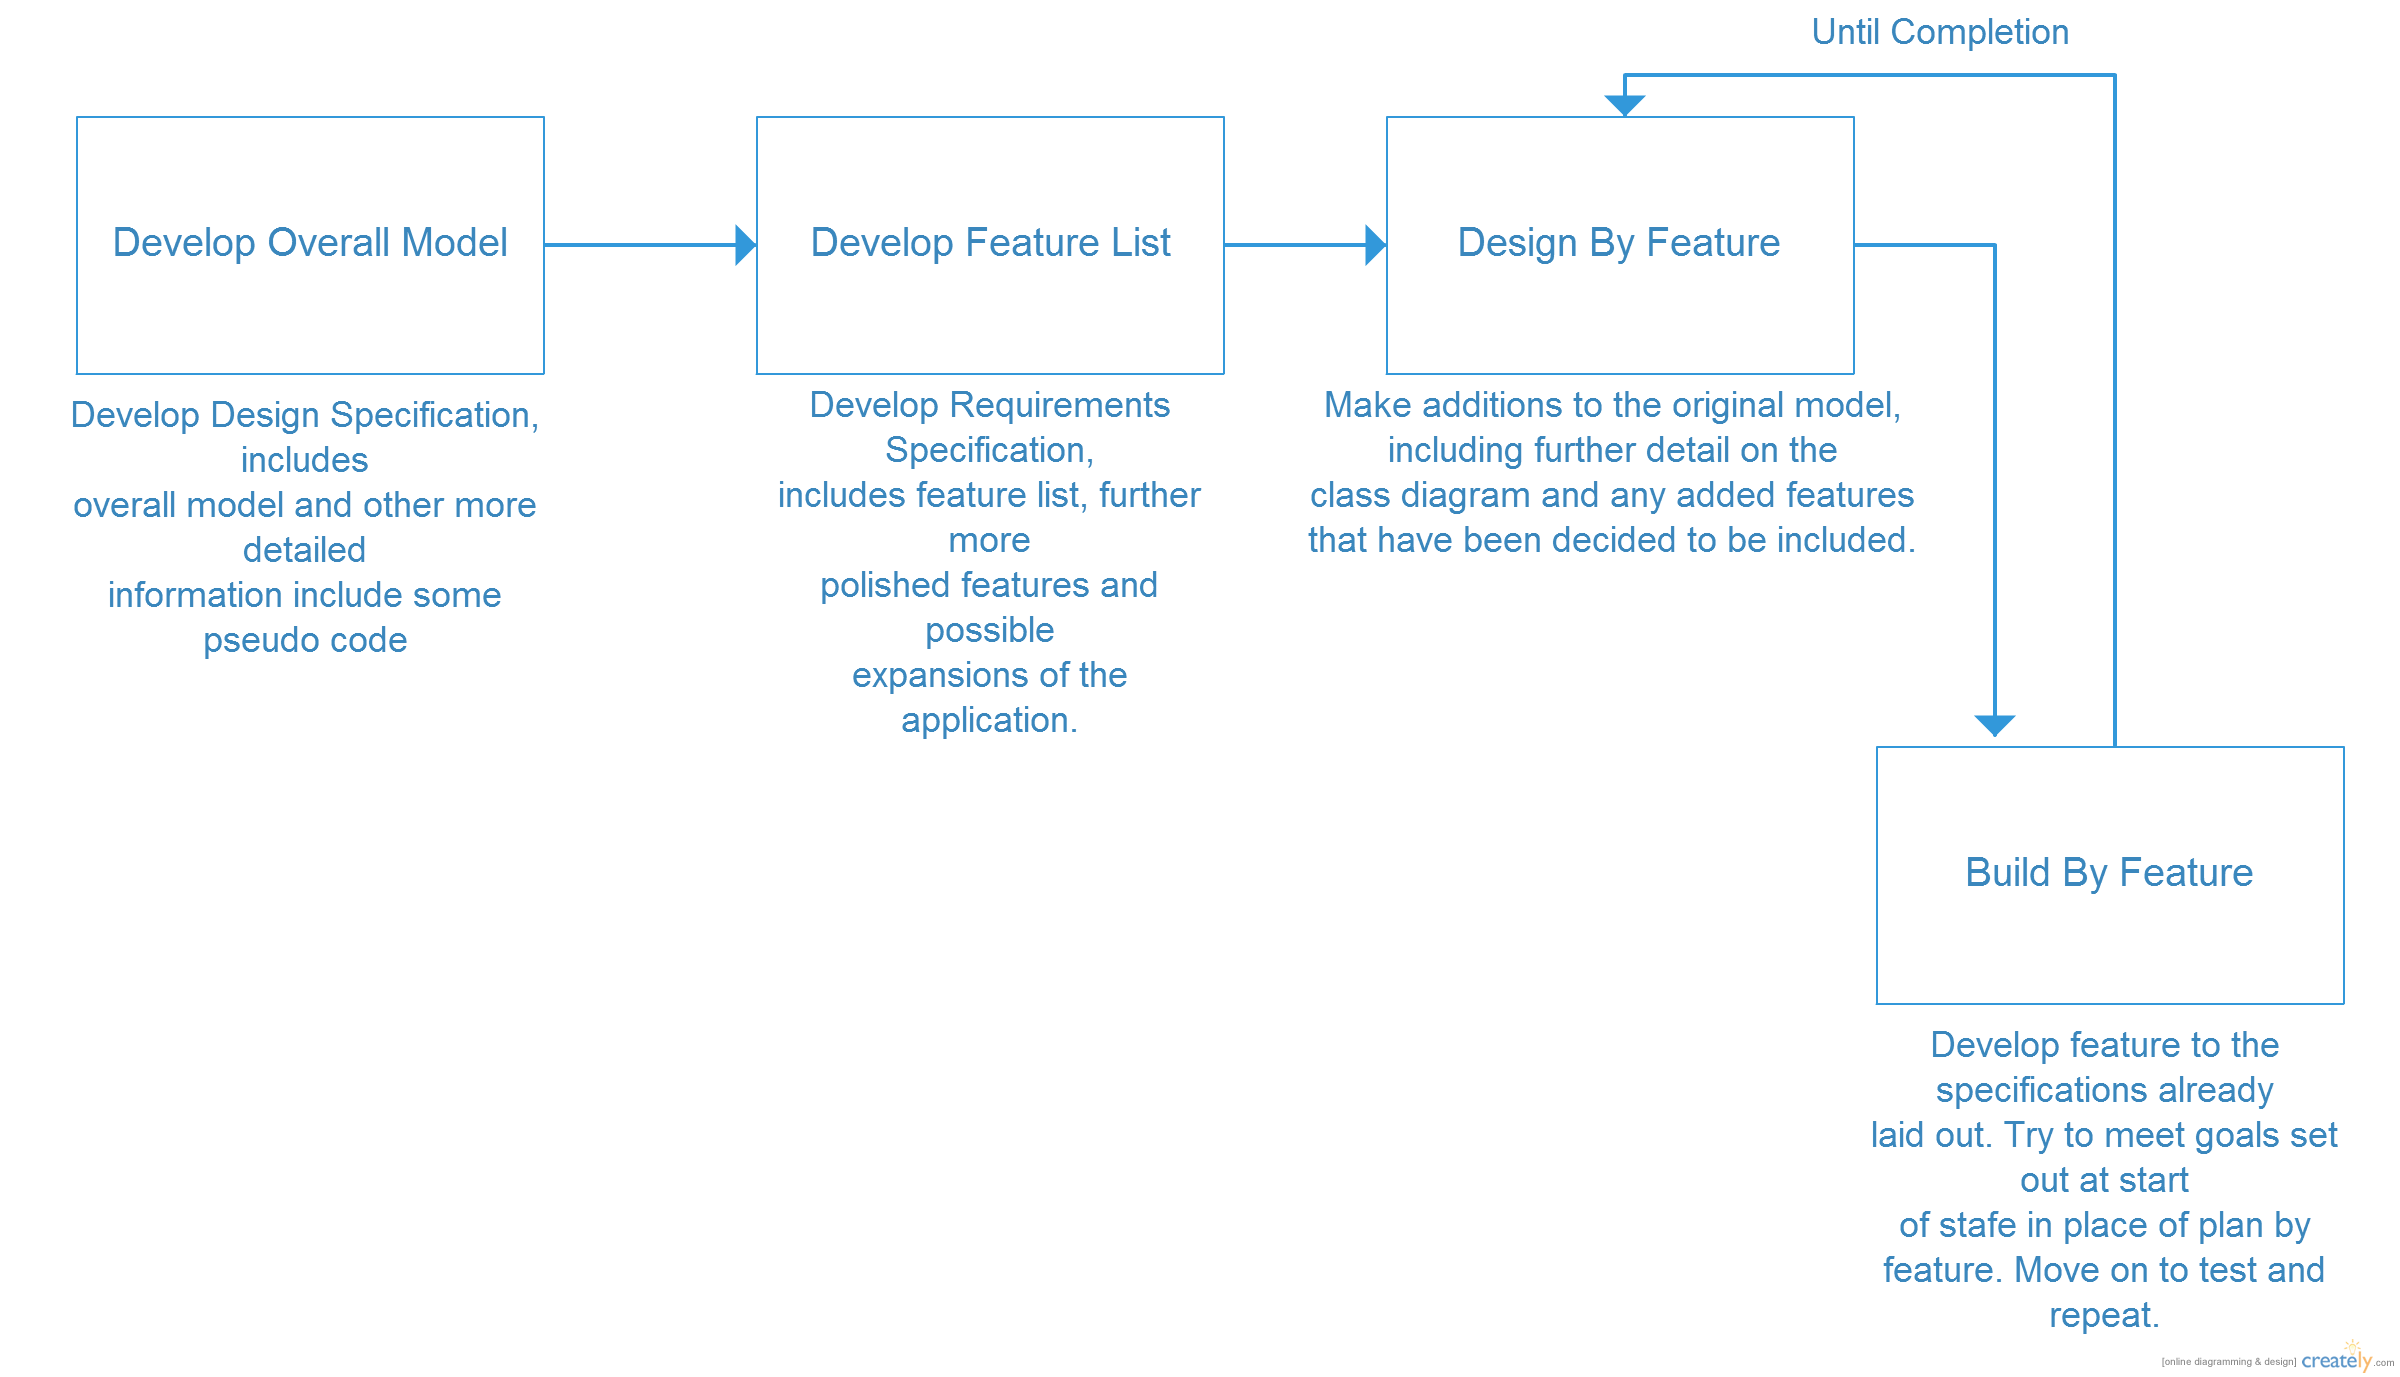
\includegraphics[scale=0.18]{Chapter1/process.png}\\
 \caption[Design Process]{Current Planned Design Process, an adapted version of FDD}
\end{figure}

